\documentclass[11pt,a4paper]{article}
\usepackage[T1]{fontenc}
\usepackage[utf8]{inputenc}
\usepackage{amsmath,amssymb,amsthm}
\usepackage{booktabs}
\usepackage{graphicx}
\usepackage{hyperref}
\usepackage{geometry}
\usepackage{longtable}
\usepackage{array}
\usepackage{url}
\geometry{margin=2.2cm}
\hypersetup{colorlinks=true,linkcolor=blue,urlcolor=blue,citecolor=blue}

\newtheorem{proposition}{Proposition}[section]
\newtheorem{lemma}[proposition]{Lemma}

\title{%
  \textbf{Online Resource 1}\\[0.5em]
  \large Algorithms, Proofs, Reproducibility Materials, and Extended Computational Results\\[1em]
  \normalsize Companion to:\\
  \textit{SCC-Local Destroy-and-Repair Heuristics for Minimum Weighted Feedback Arc Set on Sparse Digraphs}\\[0.8em]
  Computational Optimization and Applications (COAP), Springer Nature
}
\author{%
  Soroush Vahidi\thanks{Corresponding author: \texttt{sv96@njit.edu}}\\
  Department of Computer Science\\
  New Jersey Institute of Technology\\
  Newark, NJ 07102, USA
}
\date{Version 2026-06-12 \quad Source commit: \texttt{80b3144d}}

\begin{document}
\maketitle
\tableofcontents
\newpage

\section{Scope and use}
\label{sec:or1-purpose}

Online Resource~1 accompanies the COAP manuscript on SCC-local destroy-and-repair heuristics for minimum weighted feedback arc set (MWFAS) on sparse digraphs.

\subsection{Contents}

\begin{itemize}
  \item definitions and proofs, including topological-extraction inequalities (\S\ref{sec:or1-problem}, \S\ref{sec:or1-proofs});
  \item algorithm specifications and provenance (\S\ref{sec:or1-algorithms}--\S\ref{sec:or1-provenance});
  \item experiment registry EXP1--EXP11 and extended results;
  \item EXP10 stochastic-robustness evidence (\S\ref{sec:or1-exp10});
  \item EXP11 extraction-sensitivity calibration (\S\ref{sec:or1-exp11});
  \item automated tests (91 collected; \S\ref{sec:or1-tests}) and reproduction scripts.
\end{itemize}

\subsection{Claims supported}

Principal manuscript claims traceable here include: IPSNS 96/97 best observed sparse; DRMacIver 21.6\% mean excess; EXP10 median 38/55/0; 1860/1860 valid runs; exact 56/57 matches; LOLIB scope boundary; EXP11 zero extraction change on calibration subset.

\subsection{Reproduction levels}

\begin{description}
  \item[Level A--B:] seconds-scale smoke and pytest validation from included source;
  \item[Level C:] principal table verification from committed summaries (no benchmark reruns);
  \item[Level D:] optional full reruns (documented only).
\end{description}

Committed files in \texttt{results/} are authoritative for headline numbers unless a full rerun is explicitly performed.

\section{Definitions and notation}
\label{sec:or1-problem}

Let $G=(V,A,w)$ be a directed graph with vertex set $V$, arc set $A$, and nonnegative arc weights $w:A\to\mathbb{R}_{\ge 0}$.
Parallel arcs are aggregated by summing weights; self-loops are deactivated at tolerance $\tau$ when present.

A \emph{feedback arc set} (FAS) is a set $F\subseteq A$ whose removal makes $G$ acyclic.
The \emph{active DAG} is
\begin{equation}
    H=(V,A\setminus F).
    \label{eq:or1-active-dag}
\end{equation}
A \emph{vertex ordering} (linear extension) $\pi$ assigns each vertex a distinct rank.
The backward arc set induced by $\pi$ on the original graph is
\begin{equation}
    B_\pi=\{(u,v)\in A:\ \pi(v)<\pi(u)\},
    \label{eq:or1-backward-set}
\end{equation}
with ordering backward weight
\begin{equation}
    \mathrm{BW}(\pi)=w(B_\pi)=\sum_{(u,v)\in B_\pi} w(u,v).
    \label{eq:or1-bw}
\end{equation}
The removed-set weight is $w(F)=\sum_{a\in F} w(a)$.

\begin{proposition}[Backward subset and weight inequality]
\label{prop:or1-subset}
If $\pi$ is a topological order of $H$, then $B_\pi\subseteq F$. For nonnegative weights,
\begin{equation}
    \mathrm{BW}(\pi)=w(B_\pi)\le w(F).
    \label{eq:or1-inequality}
\end{equation}
\end{proposition}

\begin{proof}
Every arc of $H$ is forward under $\pi$, so no active arc belongs to $B_\pi$; hence $B_\pi\subseteq F$. Nonnegativity gives $w(B_\pi)\le w(F)$.
\end{proof}

\paragraph{Equality conditions.}
Weight equality $\mathrm{BW}(\pi)=w(F)$ holds iff $w(F\setminus B_\pi)=0$.
If every removed arc has strictly positive weight, then $\mathrm{BW}(\pi)=w(F)$ iff $B_\pi=F$.
Set equality is \emph{not} required for weight equality when zero-weight removed arcs exist.

\paragraph{Reported objective.}
Constructive methods build $(F,H)$ and extract $\pi$ by Kahn topological sorting with min-heap vertex-id tie-breaking.
Experiments report $\mathrm{BW}(\pi)$ recomputed from the returned ranking, not $w(F)$ alone.

The \emph{minimum weighted feedback arc set} (MWFAS) problem asks for an ordering minimizing $\mathrm{BW}(\pi)$; it is NP-hard in general.

\paragraph{Scope.} Sparse nonnegative weighted digraphs are the primary regime; dense LOLIB instances are a separate scope boundary.

\paragraph{Tolerances.} Implementation zero tolerance $\tau=10^{-12}$; EXP10 tie tolerance $10^{-9}$.

\section{Complete algorithm specifications}
\label{sec:or1-algorithms}

This section summarizes the implemented algorithms in \texttt{code/src/mwfas/}. Components are labeled as \textbf{inherited}, \textbf{engineered}, or \textbf{newly integrated}.

\subsection{LR-TA (inherited lineage, engineered implementation)}

\textbf{Source lineage:} Demetrescu--Finocchi local-ratio cycle reduction \cite{DF03}; engineered sparse-graph variant with recorded removals and heavy-first add-back.

\textbf{Phase I (cycle reduction):} Repeatedly detect a directed cycle $C$ in the active subgraph, compute $\varepsilon(C)=\min_{e\in C}W[e]$, subtract $\varepsilon$ from all cycle arcs, deactivate arcs with residual weight $\le\tau$.

\textbf{Phase II (add-back):} Process removed arcs in nonincreasing \emph{original} weight order. Accept forward arcs by rank shortcut; accept backward arcs only after negative reachability test; recompute topological order after backward acceptance.

\textbf{Determinism:} Phase I cycle detection uses iterative DFS with deterministic edge-index order. Floating-point subtraction may introduce tie cases handled by $\tau$.

\subsection{WMSF-style seed (inherited pipeline, engineered variant)}

\textbf{Source lineage:} Cavallaro--Cutello minimal-and-stable weighted FAS \cite{CC25}.

\textbf{Pipeline per nontrivial SCC:} \texttt{removeArcs} $\rightarrow$ \texttt{minimizeFas} $\rightarrow$ \texttt{StabilizeFas} $\rightarrow$ \texttt{minimizeFas}. Safe-edge bookkeeping restores temporarily deleted arcs. Global composition uses Kosaraju SCC decomposition.

\textbf{Note:} Stabilization may change objective; the manuscript does not claim global non-worsening for stabilization passes.

\subsection{IPSNS (newly integrated destroy-and-repair)}

\textbf{Seeds:} Run LR-TA and full WMSF seed; keep better incumbent $\pi^{(0)}$.

\textbf{Iteration $t=1,\ldots,T$:}
\begin{enumerate}
  \item Score each nontrivial SCC by backward-weight contribution under current rank.
  \item Select SCC from weighted top-$K$ pool (default $K=15$) using RNG seed.
  \item \textbf{Destroy A:} reactivate up to $\lfloor f_{\mathrm{add}}\cdot|r_S|\rfloor$ heaviest removed internal arcs.
  \item \textbf{Destroy B:} deactivate up to $\lfloor f_{\mathrm{rem}}\cdot|a_S|\rfloor$ lightest active internal arcs.
  \item \textbf{Repair:} restricted LR-TA cycle reduction + heavy-first add-back inside SCC neighborhood on original graph.
  \item Accept only if repaired ordering is acyclic and $\mathrm{BW}$ strictly improves; else exact rollback.
\end{enumerate}

\textbf{Defaults:} $T=400$, $f_{\mathrm{add}}=0.30$, $f_{\mathrm{rem}}=0.02$, $\tau=10^{-12}$, \texttt{wmsf\_seed\_mode=full}.

\subsection{Exact DP}

Bitmask dynamic programming over vertex subsets for $n\le 20$ (implementation limit). Used for exact-validation cross-checks only.

\subsection{Objective evaluation}

Independent backward-weight scan: for ordering $\pi$, sum weights of arcs $(u,v)$ with $\pi(u)>\pi(v)$. Parser and evaluator consistency is tested by the 78-test gate.

\begin{thebibliography}{9}
\bibitem{DF03} C.~Demetrescu and I.~Finocchi. Local-ratio approximation algorithms. \emph{Handbook of Approximation Algorithms and Metaheuristics}, 2007.
\bibitem{CC25} A.~Cavallaro and A.~Cutello. A minimal and stable weighted feedback arc set heuristic. \emph{Computers \& Operations Research}, 2025.
\end{thebibliography}

\section{Full proofs and formal properties}
\label{sec:or1-proofs}

Proofs correspond to Propositions in the main manuscript \S\ref{subsec:formal-analysis}. Labels indicate \emph{inherited theorem}, \emph{framework lemma}, \emph{implementation invariant}, or \emph{empirical observation}.

\subsection{LR-TA feasibility and termination}

\begin{proposition}[LR-TA feasibility and termination]
Under nonnegative original weights and the edge-indexed active-graph representation, LR-TA satisfies cycle-reduction progress, Phase~I termination in at most $m$ iterations, acyclic Phase~I output, add-back feasibility, and a valid final ordering.
\end{proposition}

\begin{proof}[Framework lemma / implementation invariant]
\textbf{(1) Cycle reduction progress.} Each Phase~I iteration selects a directed cycle $C$ and subtracts $\varepsilon(C)=\min_{e\in C}W[e]$. If $\varepsilon(C)>\tau$, at least one cycle arc reaches residual weight $\le\tau$ and is deactivated. If $\varepsilon(C)\le\tau$, the implementation deactivates one cycle arc directly. In either case at least one active arc is removed from the active subgraph.

\textbf{(2) Termination.} At most $m$ iterations occur because each iteration deactivates $\ge 1$ active arc and there are $m$ arcs initially.

\textbf{(3) Acyclic Phase~I output.} The loop stops only when no directed cycle is detected; the active subgraph is then acyclic.

\textbf{(4) Add-back feasibility.} A forward arc $(u,v)$ with $\mathrm{rank}(u)<\mathrm{rank}(v)$ cannot close a cycle upon reactivation. A backward arc is reactivated only after a reachability test certifying no $v\leadsto u$ path in the current active graph; accepted backward arcs trigger topological recomputation before later tests.

\textbf{(5) Valid ordering.} The final active graph is acyclic and yields a topological order; removed arcs define a feasible FAS under the ordering objective.
\end{proof}

\subsection{Add-back inclusion minimality}

\begin{proposition}[One-pass heavy-first add-back]
On an acyclic active graph, after every candidate removed arc has been processed once and reinserted whenever insertion preserves acyclicity, the remaining removed set is inclusion-minimal in the feedback-arc-set sense: for every remaining removed arc \(e\), restoring \(e\) to the current active DAG creates a directed cycle.
\end{proposition}

\begin{proof}[Framework lemma]
Items (1)--(3) follow from the rank and reachability arguments above. For (4), suppose arc $e=(u,v)$ remains in the removed set after the pass; then $e$ was rejected during processing, meaning a directed path $v\leadsto u$ existed in the active graph at the time of rejection. Subsequent insertions accepted in the same pass only add arcs to the active graph; adding arcs cannot destroy an existing directed path. Therefore the path $v\leadsto u$ persists after the pass completes, and $e$ cannot be reinserted into the final active graph without creating a cycle. Since every remaining removed arc was rejected for this reason, the remaining removed set is inclusion-minimal. Heavy-first ordering determines which inclusion-minimal set is obtained; it does not affect the validity of inclusion-minimality. The returned set is inclusion-minimal but not necessarily globally minimum-weight.
\end{proof}

\subsection{IPSNS incumbent protection}

\begin{proposition}[IPSNS feasibility, monotonicity, and budgeted termination]
Let $\pi^{(0)}$ be the better seed and $\pi^{(t)}$ the incumbent after iteration $t$. Then every accepted candidate is feasible, failed or non-improving moves revert exactly, $\mathrm{BW}(\pi^{(t+1)})\le \mathrm{BW}(\pi^{(t)})\le \mathrm{BW}(\pi^{(0)})$, and the loop executes at most $T$ iterations.
\end{proposition}

\begin{proof}[Implementation invariant]
(1) Acceptance requires a valid global topological order after repair. (2)--(3) The implementation snapshots activity vectors and removed sets before each move; on repair failure, infeasibility, or non-strict improvement, state is restored from the snapshot. (4) Follows from (3). (5) The outer loop counter is bounded by $T$ by construction; early stopping occurs when no nontrivial SCC has positive backward contribution.
\end{proof}

\subsection{Exact DP correctness}

\begin{proposition}[Exact DP on small instances]
For $n\le 20$ vertices, the bitmask DP enumerates all vertex orderings implicitly via subset states and returns the minimum backward weight among feasible orderings, matching brute-force enumeration on tested instances.
\end{proposition}

\begin{proof}[Implementation invariant]
The DP state records the last vertex placed and accumulated backward weight from arcs to earlier vertices in the ordering. Transitions add one vertex at a time; the minimum over full permutations is returned. The pytest gate cross-checks against independent brute force for $n\le 8$ and regression fixtures.
\end{proof}

\subsection{Qualified approximation-transfer statement}

The Demetrescu--Finocchi local-ratio framework provides approximation results under exact arithmetic and specific cycle-selection policies. The floating-point engineered implementation here does \emph{not} automatically inherit those ratio bounds; any approximation claim in the main paper is explicitly qualified as inherited literature, not re-proved for this code path.

\subsection{Topological extraction inequalities}

Proposition~\ref{prop:or1-subset} and Equations~\eqref{eq:or1-backward-set}--\eqref{eq:or1-inequality} are proved in \S\ref{sec:or1-problem}. Six independent counterexamples are automated in \texttt{tests/unit/test\_topo\_extraction\_math.py}.

\section{Algorithm provenance and implementation deviations}
\label{sec:or1-provenance-table}

\begin{table}[h]
\centering\small
\caption{Component provenance (summary). Full detail in \texttt{results/} experiment manifests.}
\begin{tabular}{p{2.2cm}p{2.5cm}p{2.5cm}p{1.5cm}p{2.8cm}}
\toprule
Component & Prior source & Current impl. & Status & Manuscript role \\
\midrule
LR-TA peeling & Demetrescu--Finocchi & \texttt{lrta.py} & Engineered & Seed \\
Topological add-back & Engineered & \texttt{lrta.py} & New integration & Dominant ablation gain \\
WMSF pipeline & Cavallaro--Cutello & \texttt{wmsf.py} & Engineered variant & Seed \\
SCC scoring & --- & \texttt{ipsns.py} & New & IPSNS selection \\
Destroy A/B & LNS literature & \texttt{ipsns.py} & New integration & IPSNS perturbation \\
Strict rollback & --- & \texttt{ipsns.py} & New & Incumbent protection \\
Exact DP & Standard & \texttt{exact.py} & Standard & Validation \\
DRMacIver wrapper & DRMacIver/FAS & external & Wrapper only & Baseline \\
\bottomrule
\end{tabular}
\end{table}

\paragraph{IPSNS novelty.} The novelty lies in the FAS-specific combination (fixed original-graph SCC neighborhoods, contribution scoring, weighted top-$K$, two-sided destroy, SCC-restricted repair, strict incumbent protection), not in generic LNS, rollback, or SCC decomposition alone.

\section{Topological-order extraction}
\label{sec:or1-topo}

Multiple topological orders may exist for an acyclic digraph. The implementation uses Kahn's algorithm with a \textbf{min-heap on vertex index} as tie-breaker: among vertices with indegree zero, the smallest vertex ID is extracted first.

\paragraph{Implications.} The extracted order is deterministic for a fixed active graph but depends on vertex numbering. Objective evaluation uses the returned order directly; no post-hoc reordering is applied.

\paragraph{Removed-set versus ordering objective.} On the final LR-TA active DAG, every positive-weight removed arc is backward under the repository extraction rule on the nonnegative calibration instances tested in EXP11; hence $w(F)=\mathrm{BW}(\pi)$ there. In general $B_\pi\subseteq F$ and $\mathrm{BW}(\pi)\le w(F)$; set equality is not required for weight equality when zero-weight removed arcs exist.

\paragraph{EXP11.} Post-hoc comparison of Kahn min-vertex-id, max-vertex-id, weighted-net priority, and one-pass precedence-preserving insertion refinement on LR-TA final active graphs found no backward-weight change on six nonnegative calibration instances; full CSV in \texttt{experiments/exp11\_topological\_extraction\_sensitivity/summary/exp11\_per\_instance.csv} (main manuscript Table~EXP11).

\paragraph{Limitation.} A different linear extension can yield a different $\mathrm{BW}(\pi)$ even for fixed $F$; the manuscript reports observed performance under the stated deterministic rule without claiming extraction optimality.

\section{Parameter provenance}
\label{sec:or1-params}

\begin{table}[h]
\centering\footnotesize
\caption{Principal parameters (defaults used in reported experiments).}
\begin{tabular}{llllp{3.5cm}}
\toprule
Parameter & Algorithm & Default & Evidence & Notes \\
\midrule
Iterations $T$ & IPSNS & 400 & EXP6 saturation & Identical mean BW at 10--400 on subset \\
top-$K$ SCC & IPSNS & 15 & Holdout & Holdout-supported default \\
$f_{\mathrm{add}}$ & IPSNS & 0.30 & Frozen & Destroy A fraction \\
$f_{\mathrm{rem}}$ & IPSNS & 0.02 & Frozen & Destroy B fraction \\
$\tau$ & All & $10^{-12}$ & Code default & Numerical safeguard \\
RNG seed & IPSNS & 1 (EXP4); 0--19 (EXP10) & EXP10 & Explicit integer seeds \\
WMSF ordering & WMSF & L2 (global) & Ablation & L1/L2 compared per SCC \\
MIP timeout & EXP8 & 120\,s & Protocol & HiGHS time cap \\
DRMacIver reps & EXP10 & 20 & Fixed & PID/time seeding \\
Tie tolerance & EXP10 & $10^{-9}$ & Fixed & Median comparison \\
\bottomrule
\end{tabular}
\end{table}

Holdout and sensitivity summaries: \texttt{results/coap\_ipsns\_sensitivity/}. EXP10 confirms the fixed IPSNS configuration showed zero cross-seed objective variation on 93/93 instances.

\section{Benchmark inventory}
\label{sec:or1-benchmarks}

Instance identifiers and participation flags are recorded in committed summaries:
\begin{itemize}
  \item \textbf{Sparse primary:} 105 instances (EXP1b internal), 97 standard nonnegative (EXP4);
  \item \textbf{Exact small:} 57 standard instances with $n\le 20$ (EXP3);
  \item \textbf{HiGHS MIP:} 15 medium instances, $n\le 318$ (EXP8);
  \item \textbf{LOLIB dense:} 50 complete ordering instances (EXP5);
  \item \textbf{EXP10 common subset:} 93 instances (manifest \texttt{manifests/common\_93\_instances.txt}).
\end{itemize}

Per-instance vertex counts, arc counts, densities, and checksums appear in \texttt{results/exp4/summary/exp4\_raw\_summary.csv}, \texttt{results/exp10/summary/paired\_median\_comparison.csv}, and related files. Public sources: graph-benchmarks repository and LOLIB (URLs in main manuscript).

\paragraph{Handling.} The sparse input list contained 123 paths; duplicate basenames were collapsed by keeping the first listed path for each instance name, yielding 105 unique instances. Nonnegative sparse standard set excludes eight negative-weight instances. DIMACS files are parsed line by line: comment and problem lines are ignored, parallel arcs are aggregated by summing weights, self-loops are retained if present, malformed arc records are skipped, and isolated vertices appear only when referenced by arcs. Checksums and per-instance \((n,m)\) values appear in \texttt{results/exp4/summary/exp4\_raw\_summary.csv} and related files.

\section{Complete experimental protocol}
\label{sec:or1-protocol}

\paragraph{Hardware/software.} Linux workstation, Intel Core i7-12700K, 62\,GiB RAM, Ubuntu 24.04, Python 3.12.3. Package versions: \texttt{environment/dependency\_lock\_or\_freeze.txt}.

\paragraph{External tools.} DRMacIver/FAS binary SHA-256: \texttt{907b7abe96ff8fb54d8b70910eb3068744f765e72da5520f2c7aacf70ba996bd}. python-igraph 1.0.0 for Eades wrapper. HiGHS for EXP8.

\paragraph{Seeds and checkpoints.} IPSNS uses explicit integer seeds. DRMacIver repetitions inherit PID/time-based seeding in the external executable. EXP10 uses atomic JSON writes, checkpoint \texttt{.done} files, and validation before analysis.

\paragraph{Failure handling.} Failed, timed-out, or malformed runs are retained and reported; no silent reruns until success.

\paragraph{Statistics.} EXP4/EXP10 paired tests use SciPy 1.17.1 \texttt{scipy.stats.wilcoxon} with \texttt{alternative="two-sided"} and \texttt{zero\_method="wilcox"}, plus a two-sided sign test excluding ties. Bootstrap CI uses seed 42 and 10,000 resamples. \emph{IPSNS comparator-normalized reduction} is the mean of $(X-\mathrm{IPSNS})/X\times 100$ over instances with $X>0$; zero-zero pairs contribute 0\%. Exact-validation mean gap uses $(\mathrm{BW}_{\mathrm{heuristic}}-\mathrm{BW}_{\mathrm{opt}})/\mathrm{BW}_{\mathrm{opt}}\times 100$ with zero-optimum instances assigned gap 0 when the heuristic also attains optimum 0.

\paragraph{Runtime.} Wall-clock per instance; includes parsing and conversion where stated. EXP10 comparison is quality-focused, not equal-time.

\section{Extended computational results}
\label{sec:or1-extended}

Committed summaries supporting the main manuscript tables:

\begin{table}[h]
\centering\small
\caption{Principal manuscript numbers and OR1 source files.}
\begin{tabular}{ll}
\toprule
Claim & Source file \\
\midrule
96/97 IPSNS best (sparse) & \texttt{results/exp4/summary/exp4\_external\_stats.json} \\
21.61\% IPSNS mean reduction relative to DRMacIver/FAS & same \\
56/57 exact matches & \texttt{results/exp3/summary/exp3\_exact\_stats.json} \\
0 incumbent violations (105) & \texttt{results/exp1/summary/exp1b\_core\_benchmark\_stats.json} \\
5.9\% add-back ablation & \texttt{results/exp2/summary/exp2\_ablation\_stats.json} \\
LOLIB 45 DRMacIver wins & \texttt{results/exp5/summary/exp5\_lolib\_stats.json} \\
HiGHS 7/15 optimal & \texttt{results/exp8/summary/exp8\_mip\_summary.json} \\
\bottomrule
\end{tabular}
\end{table}

Full per-instance CSV tables: \texttt{results/combined/tables/}, \texttt{results/exp4/summary/exp4\_raw\_summary.csv}, and experiment-specific \texttt{tables/} directories. Regenerate via \texttt{scripts/reproduce\_principal\_tables.sh}.

\subsection{Material condensed from the main manuscript}

The revised main paper keeps only the claim-bearing tables needed for the IPSNS-centered sparse narrative. The following supporting items are therefore documented here.

\begin{itemize}
  \item \textbf{EXP4 paired sparse tests:} full win/tie/loss and paired-test summaries for IPSNS against all baselines remain in \texttt{results/exp4/tables/} and the manuscript table source \texttt{paper\_coap/tables/table\_paired\_sparse\_tests.tex}.
  \item \textbf{EXP6 budget study:} the full quality-versus-budget table and curve are retained in \texttt{paper\_coap/tables/table\_ipsns\_budget\_curve.tex} and the corresponding figure assets; source summaries are in \texttt{results/exp6/summary/}.
  \item \textbf{EXP7 local-search controls:} detailed adjacent-swap and insertion-local-search comparisons remain in \texttt{paper\_coap/tables/table\_plain\_local\_search.tex} and \texttt{results/exp7/summary/}.
  \item \textbf{EXP8 medium MIP details:} per-instance certification outcomes remain in \texttt{results/exp8/summary/exp8\_mip\_summary.json}; the compact manuscript table source is \texttt{paper\_coap/tables/table\_medium\_mip\_baseline.tex}.
  \item \textbf{EXP9 application example:} the public ordering example remains in \texttt{paper\_coap/tables/table\_application\_case.tex} with supporting summaries in \texttt{results/exp9/summary/}.
  \item \textbf{EXP11 extraction sensitivity:} the full calibration table remains in Section~\ref{sec:or1-exp11}.
  \item \textbf{Structural diagnostics:} sparse-versus-dense density and SCC summaries remain in \texttt{paper\_coap/tables/table\_structural\_diagnostic.tex} and the associated summary files.
\end{itemize}

\paragraph{Rows moved from the compact main-paper tables.}
The compact ablation table in the manuscript omits the secondary control ``IPSNS, no SCC priority'', whose archived values are mean BW \(4239.1\), relative change \(-0.76\%\), and mean runtime \(5.727\) s on the 10-instance subset. The compact LOLIB table also omits family-level detail: IPSNS versus DRMacIver/FAS best counts are \(1/25\) versus \(24/25\) on SGB, \(4/10\) versus \(6/10\) on IO, and \(0/15\) versus \(15/15\) on RandA1, with mean BW pairs \(1{,}048{,}056 / 1{,}036{,}085\), \(36{,}996 / 32{,}860\), and \(169{,}755 / 156{,}909\), respectively.

\begin{table}[h]
\centering\small
\caption{Ablation table moved from the main paper. Relative change is measured against LR-TA.}
\begin{tabular}{lrrr}
\toprule
Variant & Mean BW & Relative change & Mean RT (s) \\
\midrule
LR without add-back & 4525.1 & +5.94\% & 0.017 \\
LR-TA & 4271.5 & +0.00\% & 0.047 \\
WMSF seed & 4332.5 & +1.43\% & 0.040 \\
Best seed, no refinement & 4271.5 & +0.00\% & 0.069 \\
IPSNS, 50 iterations & 4239.2 & -0.76\% & 0.778 \\
IPSNS, 400 iterations (default) & 4239.2 & -0.76\% & 5.734 \\
IPSNS, no SCC priority & 4239.1 & -0.76\% & 5.727 \\
\bottomrule
\end{tabular}
\end{table}

\subsection{Holdout-supported defaults}

The IPSNS default settings reported in the main paper are supported by the archived holdout study under \texttt{experiments/coap\_ipsns\_holdout/}. The study contains 18 tuning instances, 25 holdout instances, six configurations, and five seeds per configuration-instance pair (1290 completed runs). The committed aggregate summary records zero incumbent violations and identical holdout median final BW across the tested configurations, so the defaults are treated as engineering choices rather than as uniquely optimal tuned parameters.

\section{EXP10 stochastic robustness}
\label{sec:or1-exp10}

\subsection{Design}

93-instance common sparse subset; 20 IPSNS seeds (0--19); 20 DRMacIver/FAS repetitions per instance. Production records: 1860+1860 validated (0 failures). Smoke artifacts excluded.

\subsection{Primary median comparison}

\begin{center}
\begin{tabular}{lr}
\toprule
Metric & Value \\
\midrule
IPSNS wins / ties / DR wins & 38 / 55 / 0 \\
Mean relative excess (DR over IPSNS) & 21.60\% \\
Wilcoxon $p$ (two-sided) & $<0.001$ \\
Sign test $p$ (two-sided) & $<0.001$ \\
Cohen's $d_z$ & $-0.31$ \\
\bottomrule
\end{tabular}
\end{center}

\subsection{Variability}

IPSNS: zero objective variation on 93/93 instances; seed 0 matched best on all 93. DRMacIver: 40/93 instances with multiple distinct objectives; 1860 unique PIDs.

\subsection{\texttt{r20\_60} reversal}

EXP4 single run: DRMacIver 1685 vs IPSNS 1688 (DR win). EXP10 medians: IPSNS 1688 vs DRMacIver 1698 (IPSNS win).

\subsection{Warnings}

\begin{itemize}
  \item Zero IPSNS cross-seed variance documents empirical stability under the frozen configuration; it does \textbf{not} prove mathematical determinism.
  \item The repeated-run comparison is \textbf{not} equal-time; DRMacIver intermediate solutions are unavailable.
\end{itemize}

\subsection{Figures and tables}

\begin{figure}[h]
\centering
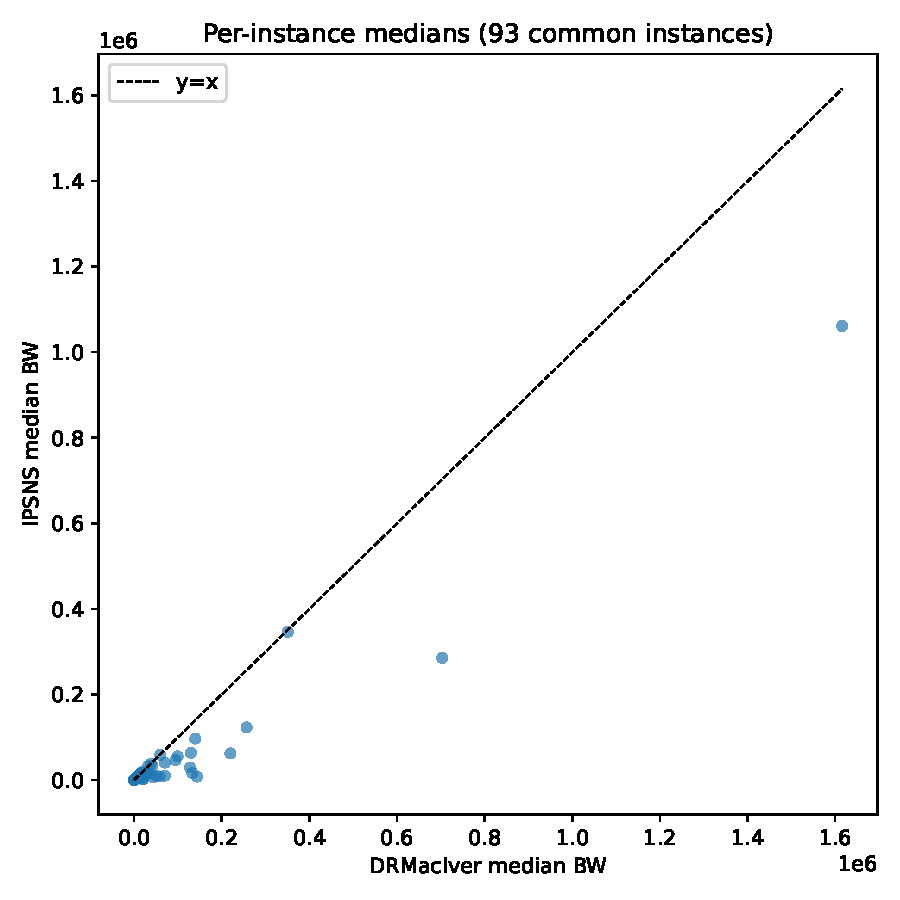
\includegraphics[width=0.55\textwidth]{figures/exp10_median_scatter.pdf}
\caption{EXP10 per-instance medians (93 instances).}
\end{figure}

Complete tables: \texttt{results/exp10/summary/paired\_median\_comparison.csv}, \texttt{best\_of\_k.csv}, \texttt{probability\_of\_win.csv}. Figures: \texttt{results/exp10/figures/}.

\section{EXP11: topological-extraction sensitivity}
\label{sec:or1-exp11}

EXP11 is a post-hoc calibration study on LR-TA final active DAGs. It does not modify LR-TA, WMSF, IPSNS, or any headline benchmark output.

\subsection{Motivation}
Linear extensions of a fixed active DAG are not unique; $\mathrm{BW}(\pi)$ can depend on the extraction rule (Proposition~\ref{prop:or1-subset}, Equation~\eqref{eq:or1-inequality}). EXP11 tests whether alternative deterministic extractions change reported backward weight on a small nonnegative calibration subset.

\subsection{Frozen protocol}
\begin{itemize}
    \item \textbf{Instances:} six nonnegative calibration graphs (\texttt{bad1}, \texttt{gr10}, \texttt{s420}, \texttt{s349}, \texttt{s641}, \texttt{example.new}).
    \item \textbf{State:} LR-TA final $(F,H)$ reconstructed from source (active flags not stored in committed summaries).
    \item \textbf{Rules:} (i)~repository Kahn min-vertex-id; (ii)~Kahn max-vertex-id; (iii)~Kahn weighted net-score priority; (iv)~one-pass precedence-preserving insertion refinement respecting active-DAG precedence.
    \item \textbf{Metrics:} $\mathrm{BW}(\pi)$, $w(F)-\mathrm{BW}(\pi)$, relative improvement with $\varepsilon=10^{-9}$.
    \item \textbf{Runtime:} ${\sim}9$\,s on the frozen subset (source commit in front matter).
\end{itemize}

An exploratory broader run was stopped before completion; the first insertion-refinement prototype did not enforce active-DAG precedence and was corrected before the frozen valid run recorded here.

\subsection{Results}
\begin{center}
\begin{tabular}{lrrr}
\toprule
Instance & $\mathrm{BW}(\pi)$ (all rules) & $w(F)-\mathrm{BW}(\pi)$ & Improved? \\
\midrule
bad1 & 94 & 0 & no \\
gr10 & 62\,435 & 0 & no \\
s420 & 158 & 0 & no \\
s349 & 6\,729 & 0 & no \\
s641 & 2\,403 & 0 & no \\
example.new & 18\,638 & 0 & no \\
\bottomrule
\end{tabular}
\end{center}

\textbf{Conclusion:} zero backward-weight changes; zero headline impact on EXP4/EXP10 comparisons. Full CSV: \texttt{results/exp11/summary/exp11\_per\_instance.csv}.

\paragraph{Limitation.} Six-instance calibration only; does not prove extraction optimality on the full 97-instance benchmark.

\section{Automated tests}
\label{sec:or1-tests}

The artifact includes the current pytest gate (\texttt{tests/}, \texttt{src/mwfas/}).

\begin{center}
\begin{tabular}{lr}
\toprule
Metric & Count \\
\midrule
Collected & 86 \\
Passed & 79 \\
Skipped & 7 \\
Failed & 0 \\
Errors & 0 \\
\bottomrule
\end{tabular}
\end{center}

\textbf{History.} The full repository gate collects 91 tests (90 passed, 1 skipped after EXP11). The packaged OR1 archive excludes live EXP10 production scripts/checkpoints; its pytest summary is 79 passed, 7 skipped (86 collected) because EXP10 namespace tests skip when the live experiment tree is absent.

\textbf{Full-repository command:} \texttt{PYTHONPATH=src python3 -m pytest tests/ -q} from the complete checkout yields 90 passed, 1 skipped.

\textbf{Command:} \texttt{PYTHONPATH=src python3 -m pytest tests/ -q}

\textbf{Categories:} objective equivalence; $B_\pi\subseteq F$ and weight inequalities; topological extraction counterexamples; I/O parser contracts; LR-TA feasibility; WMSF safe-edge regression; IPSNS rollback; exact DP; CLI smoke; EXP10 namespace patterns.

\paragraph{Limitation.} Tests certify implementation behavior on small graphs; they do not constitute formal verification.

\section{Reproduction instructions}
\label{sec:or1-reproduce}

\subsection{Level A --- Smoke validation}

\begin{verbatim}
./scripts/reproduce_smoke.sh
\end{verbatim}
Runs LR-TA, exact DP, and topological fixtures on bundled tiny graphs.

\subsection{Level B --- Test suite}

\begin{verbatim}
./scripts/reproduce_tests.sh
\end{verbatim}
Expected pytest summary: \textbf{90 passed, 1 skipped} (91 collected).

\subsection{Level C --- Principal table verification}

\begin{verbatim}
./scripts/reproduce_principal_tables.sh
\end{verbatim}
Verifies EXP4, EXP3, EXP10, EXP11, and combined manuscript tables from committed summaries.

\subsection{Level D --- Full rerun (optional)}

See \texttt{scripts/optional\_full\_reproduction.sh}. Requires external datasets and binaries; not part of ordinary validation.

\subsection{Artifact validation}

\begin{verbatim}
./scripts/validate_artifact.sh
\end{verbatim}

\section{Limitations}
\label{sec:or1-limits}

\begin{itemize}
  \item \textbf{Sparse specialization:} strongest claims apply to sparse nonnegative weighted digraphs.
  \item \textbf{Dense LOLIB:} matrix-based DRMacIver/FAS is stronger on complete ordering instances.
  \item \textbf{No universal SOTA claim:} comparisons are relative to the evaluated method set.
  \item \textbf{Incomplete solver ecosystem:} several literature methods lack accessible weighted implementations in the same pipeline.
  \item \textbf{Topological-order dependence:} linear extensions are not unique; EXP11 found no backward-weight change on a six-instance calibration subset but does not prove extraction optimality globally.
  \item \textbf{Floating-point:} tolerance-qualified guarantees only.
  \item \textbf{EXP10 interpretation:} IPSNS zero variance is empirical; DRMacIver is restart-sensitive; not equal-time.
  \item \textbf{External binary nondeterminism:} DRMacIver seeding is not author-controlled.
  \item \textbf{Hardware:} runtimes may differ across machines.
  \item \textbf{Terminology:} ``best observed'' $\neq$ certified optimum except on stated exact/MIP subsets.
\end{itemize}

See also \texttt{provenance/known\_limitations.md}.


\end{document}
